\section{Teorema de Arnold-Liouville}\label{sec:arnoldliouville}
A la hora de estudiar sistemas dinámicos, una cuestión interesante a plantearse, con consecuencias prácticas y también de carácter fundamental, es si las ecuaciones del sistema podrán ser «integradas», es decir, si podrán ser resueltas mediante integrales («cua\-dra\-tu\-ras») de funciones conocidas. Decimos entonces que una ecuación diferencial es \emph{integrable por cuadraturas} si es posible escribir su solución general en términos de sumas, productos, composiciones e integrales de funciones conocidas. 

En 1885, Joseph Liouville encontró una condición necesaria para que las ecuaciones de Hamilton de ciertos sistemas hamiltonianos fueran (localmente) integrables por cuadraturas. Décadas más tarde, con la introducción del formalismo geométrico y topológico al estudio de los sistemas dinámicos se descubrirían muchas más cosas interesantes sobre los sistemas que cumplían la condición que Liouville propuso. Destaca especialmente en todo este estudio la teoría de los toros invariantes desarrollada por Vladimir Arnold en 1963. Nace así la teoría de los \emph{sistemas integrables}, cuyos resultados más básicos constituyen el \emph{teorema de Arnold-Liouville}.

\begin{defn}\label{integrable}
  \em
  Sea $(M,H)$ un sistema hamiltoniano con $\dim(M)=2n$. Decimos que $(M,H)$ es \emph{integrable (en el sentido de Liouville)} si existen $F_1,\dots,F_n\in \mathscr{C}^{\infty}(M)$ que
\begin{enumerate}
  \item son \emph{funcionalmente independientes}, es decir, $\dd F_{1,x}\wedge \dots \wedge \dd F_{n,x}\neq 0$ para casi todo punto\footnote{Como aquí en principio no estamos considerando ninguna medida, con \emph{para casi todo punto} queremos decir en un conjunto \emph{residual} o \emph{comagro}, esto es, que su complementario sea \emph{magro}. Un conjunto se dice \emph{magro} o \emph{de primera categoría de Baire} si es unión numerable de conjuntos diseminados, esto es, de conjuntos cuya adherencia tiene interior vacío. Por ejemplo, el conjunto de los números racionales $\mathbb{Q}\subset\RR$ no es diseminado pero sí es magro en $\RR$. } $x\in M$, 
  \item están \emph{en involución}, esto es, $\pois{F_i}{F_j}=0$ para cada $i,j=1,\dots,n$, y
  \item  los campos $X^{F_i}$ son completos para cada $i=1,\dots,n$. 
\end{enumerate}
En particular, si $F_1=H$, todas las funciones $F_1,\dots,F_n$ son integrales primeras del sistema.

Si escribimos $F:M\rightarrow \RR^n$ con $F(x)=(F_1(x),\dots,F_n(x))$. Los puntos $x\in M$ en los que $\mathrm{rango} (\dd F_x) =n$ se llaman \emph{puntos regulares} del sistema. Los puntos que no son regulares se llaman \emph{puntos críticos}. Si $x\in M$ es un punto crítico, $F(x)$ se llama \emph{valor crítico}. Por tanto, llamamos \emph{valores regulares} a los valores que no son críticos, es decir, a aquellos $a\in \RR^n$ tales que si $a=F(x)$, entonces $x$ es un punto regular. Si $\Sigma$ es el conjunto de los puntos críticos, el conjunto de los valores críticos $F(\Sigma)\in \RR^n$ se llama \emph{diagrama de bifurcación} del sistema.
Nótese que, por el teorema de Sard\footnote{El teorema de Sard afirma que si $\Sigma$ denota el conjunto de puntos críticos de una función $f\in \mathscr{C}^k(\RR^n,\RR^m)$, con $k\geq \text{máx}\left\{ n-m+1,1 \right\}$ entonces su imagen $f(\Sigma)$ tiene medida nula.}, el diagrama de bifurcación tiene medida nula.
\end{defn}

\begin{obs}
  \em
  De la definición y de la conservación de la energía directamente se deduce que todo sistema con un grado de libertad (y cuyo hamiltoniano sea regular en casi todo punto) es integrable en el sentido de Liouville. Asimismo, un sistema con dos grados de libertad que tenga una cantidad conservada independiente de la energía también será integrable en el sentido de Liouville, ya que las cantidades conservadas dan 0 al evaluar el corchete de Poisson de cada una de ellas con el hamiltoniano.
\end{obs}

\begin{thm}[Arnold-Liouville]\label{arnold}
  Sea $(M,H)$ un sistema integrable en el sentido de Liouville con $F_1(=H),\dots,F_n$ las integrales primeras en involución. Sea $a$ un valor regular y el conjunto de nivel $F^{-1}(a)$. Sea $x\in F^{-1}(a)$ y $M_a$ la componente conexa de $F^{-1}(a)$ que contiene a $x$.  Entonces:

$1$. $M_a$ es una variedad diferenciable invariante bajo el flujo del sistema y $\left. \omega \right|_{M_a}=0$.
  
$2$. $M_a$ es difeomorfa a $\TT^k\times \RR^{n-k}$ para cierto $0 \leq k \leq n$. En particular, si $M_a$ es compacta, $M_a$ es difeomorfa al toro $n$-dimensional $\TT^n$. En este caso, se dice que $M_a$ es un \emph{toro de Liouville}. 
 
$3$. Podemos tomar unas coordenadas $w=(w_1,\dots, w_n)$ en $M_a$ de manera que existen unas velocidades constantes $v(a)=(v_1(a),\dots,v_n(a))$ tales que $\dot w (t)=v(a)$. 
\end{thm}

 \begin{proof}
  En primer lugar, como $F$ tiene rango máximo en cada punto de $M_a$, por el teorema de la función implícita $M_a$ es una subvariedad regular de $M$ de dimensión $2n-n=n$. 
  Como $M$ es una variedad simpléctica, para cada $i=1,\dots,n$, podemos definir el campo $X_i=X^{F_i}$. Al ser las $\dd F_i$ linealmente independientes los campos $X_i$ son linealmente independientes. Además, por \ref{proppoisson}, como para cada $i,j= 1,\dots,n$ $\pois{F_i}{F_j}=0$, tenemos que $\lie{X_i}{X_j}=0$ y que $\omega(X_i,X_j)=0$. Por esto mismo, la derivada de la función $F_i$ en la dirección de $X_j$ es 0, luego los campos $X_j$ son tangentes a $M_a$.

  De aquí sacamos varias conclusiones:
  \begin{enumerate}
    \item $M_a$ es invariante con respecto a cada uno de los $n$ flujos hamiltonianos generados por cada función $F_i$ (luego, en particular lo será respecto del generado por $F_1$).
    \item Como, para cada $x \in M_a$, los vectores $X_1|_x,\dots, X_n|_x$ forman una base de $T_x M_a$, $\omega$ se anula en $T_x M_a$. 
    \item $M_a$ es una variedad diferenciable de dimensión $n$ con $n$ campos conmutativos dos a dos y linealmente independientes en todo punto de $M_a$. 
  \end{enumerate}

  Esto prueba la parte $1$ del teorema. Para continuar, necesitamos probar un lema previo.

  \begin{lema}\label{lemtoro}
    Sea $N$ una variedad diferenciable de dimensión $n$ conexa tal que existen campos $X_1,\dots,X_n$ en $N$ completos y linealmente independientes y tales que, para $i\neq j$, $[X_i,X_j]=0$. Entonces $N$ es difeomorfa a $\TT^k\times \RR^{n-k}$. 
\end{lema}
\begin{proof}
  Para cada $i=1,\dots,n$, sea $g_i$ el flujo completo generado por $X_i$. Como para todo $i\neq j$, $[X_i,X_j]=0 $, entonces $g_i$ conmuta con $g_j$, es decir, $g_{i,t}g_{j,s} (x)=g_{j,s}g_{i,t} (x)$, para todo $x \in N$. 

  Así, podemos definir una acción de $\RR^n$ en $N$ que a cada $t=(t_1,\dots,t_n)\in \RR^n$ le asigna $g_t:N\rightarrow N,$ con $g_t=g_{1,t_1}\cdots g_{n,t_n}$.
Por conmutar los flujos, $g_{t+s}=g_t g_s$. Ahora, fijo $x_0 \in N$, definimos 
\[
  \begin{array}{rcl}
g:\RR^n & \longrightarrow & N \\
t & \longmapsto & g_t (x_0).
\end{array}
\]

Como los campos son linealmente independientes, $d_t g$ es un isomorfismo lineal para todo $t$ y, por el teorema de la función inversa, $g$ es un difeomorfismo local. Ahora, dado $x\in N$, tomamos una curva $\gamma$ en $N$ que una $x$ y $x_0$. Por ser $g$ un difeomorfismo local, para todo $y\in \gamma$ existe un entorno $U$ de $y$ tal que $g_t(y)$ da un difeomorfismo entre $U$ y un entorno $W\in \RR^n$ centrado en $0$. Por ser $\gamma$ compacta, podemos tomar entonces una sucesión finita de entornos $U_0,\dots,U_r$ que recubran $\gamma$ tales que $x_0 \in U_0$ y $x \in U_r$ y tales que existan unos puntos $x_1,\dots,x_r$ pertenecientes a $U_1,\dots,U_r$, respectivamente, con $x_r=x$, de forma que $g_t(x_i)$ dé un difeomorfismo entre un entorno $W_i\subset \RR^n$ centrado en $0$ y $U_i$. Tomemos ahora unos puntos $y_1,\dots,y_{r}$ pertenecientes a $U_0\cap U_1,\dots,U_{r-1}\cap U_r$, respectivamente. Entonces, para cada $i=1,\dots,r$, $y_i=g_{s_i}(x_{i-1})=g_{t_i}(x_{i})$, para ciertos $s_i, t_i \in \RR^n$, luego $x_{i}=g_{s_i-t_i}(x_{i-1})$. Por tanto, 
$$x=x_{r}=g_{s_{r}-t_{r}}(x_{r-1})=g_{s_{r}-t_{r}+s_{r-1}-t_{r-1}+\cdots+s_1-t_1}(x_0).$$ De modo que $g$ es sobreyectiva.

\begin{figure}[h!]
  \centering
  \includegraphics[width=0.8\textwidth]{pics/entornos.eps}
  \caption{\small Idea de la demostración de que $g$ es sobreyectiva.}
  \label{fig:entornos}
\end{figure}

Tenemos entonces que $g:\RR^n\rightarrow N$ es un difeomorfismo local sobreyectivo, luego es una identificación diferenciable. Denotamos 
\[  
  \Gamma:=\{t \in \RR^n \mid g_t(x_0)=x_0\},
\]
que es un subgrupo de $(\RR^n,+)$ ya que, dados $t, s \in \Gamma$, 
\[
  g_{s+t}(x_0)=g_sg_t(x_0)=g_s(x_0)=x_0
\]
y 
\[
  g_{-t}(x_0)=g_{-t}g_t(x_0)=x_0.
\] 
 Además, $\Gamma$ no depende de la elección de $x_0$, en efecto, si $x=g_s (x_0)$ y $t\in \Gamma$, entonces 
\[
  g_t (x) = g_{t+s}(x_0)=g_sg_t(x_0)=g_s(x_0)=x. 
 \] 
Ahora, por la propiedad universal del cociente, si $\pi:\RR\rightarrow \RR^n/\Gamma$ denota la proyección natural, el siguiente diagrama
\begin{center}
  \begin{tikzcd}
    \RR^n \arrow{r}{g}\arrow{d}[anchor=west]{\pi} & N    \\ 
    \RR^n/\Gamma, \arrow{ru}[anchor=north,rotate=30]{\tilde{g}}
  \end{tikzcd}
\end{center}
da un difeomorfismo $\tilde{g}:N\rightarrow \RR^n/\Gamma$. Si $\Gamma=\{0\}$, entonces $g:N\rightarrow \RR^n$ es un difeomorfismo y habríamos terminado. Supongamos que $\Gamma \neq\left\{ 0 \right\}$.

 Como $g$ es un difeomorfismo local, existe un entorno $V\subset \RR^n$ de 0 tal que $\Gamma\cap V= \{0\}$. Es más, si $t\in \Gamma$, $s\in V\backslash \{0\}$ y $x\in N$, 
  \[
    g_{t+s}(x)=g_sg_t(x)=g_s(x)\neq x.
  \]
  Luego $\Gamma$ es un conjunto discreto. Nótese también que $\Gamma$ es cerrado en $\RR^n$.
  \begin{figure}[h]
    \centering
    \includegraphics[width=0.25\textwidth]{pics/discreto}
    \caption{\small Idea de que $\Gamma$ es discreto.}
    \label{fig:discreto}
  \end{figure}

  Antes de continuar, es necesario probar el siguiente lema:
  \begin{lema}\label{discreto}
    Todo subgrupo no trivial, cerrado y discreto $\Gamma$ de $\RR^n$ es isomorfo a $\ZZ^k$ para algún $k\in\{1,\dots,n\}$. Es decir, existen $e_1,\dots,e_k \in \Gamma$ linealmente independientes tales que 
    \[
      \Gamma=\{n_1e_1+\cdots+n_ke_k \mid (n_1,\dots,n_k) \in \ZZ^k \}.
    \]
  \end{lema}
  \begin{proof}
  Sea $e_0 \in \Gamma$, $e_0 \neq 0$. Como $\Gamma$ es discreto, $\Gamma \cap D(0,\norm{e_0})$ (donde $D(a,r)$ denota el disco cerrado de centro $a$ y radio $r$) es finito. De estos puntos consideramos aquellos que están en $L(e_0)$ \footnote{Aquí $L(x)$ denota la envoltura lineal de $x$.} y de estos escogemos el más cercano, que llamaremos $e_1$. 
  
  Si existieran algún $e \in \Gamma$ y algún $m \in \ZZ$ tal que $e \in (me_1,(m+1)e_1)$, entonces $e-me_1 \in \Gamma \cap L(e_0)$ estaría más cerca de 0 que $e_1$. Por tanto, 
  \[
   \Gamma\cap L(e_0) = e_1\ZZ.
  \]

  Si no hay puntos de $\Gamma$ fuera de $L(e_1)$ hemos terminado, $\Gamma$ es isomorfo a $\ZZ$. En caso contrario, dado $e \in \Gamma \backslash L(e_1)$, proyectamos ortogonalmente $e$ sobre $L(e_1)$. Esta proyección cae exactamente sobre un intervalo $\Delta=[me_1,(m+1)e_1)$ para cierto $m \in \ZZ$. Sea $C$ el cilindro cerrado de eje $\Delta$ y de radio igual a la distancia entre $\Delta$ y $e$. $C\cap \Gamma$ es finito, y de sus puntos, sea $e_2$ el más cercano a $\Delta$ que no esté en $\Delta$. Entonces, para cualquier otro $f \in \Gamma$, la distancia entre $f$ y $L(e_1)$ es mayor que la distancia entre $e_2$ y $L(e_1)$. 
    
    En efecto, si existe $l \in \ZZ$ tal que la proyección ortogonal de $f$ cae sobre $[le_1,(l+1)e_1)$, entonces $f'=f-le_1+me_1 \in C$ y la distancia entre $f'$ y $L(e_1)$ es menor que la distancia entre $e_2$ y $L(e_1)$, lo que nos lleva a una contradicción.

  \begin{figure}[h]
    \centering
    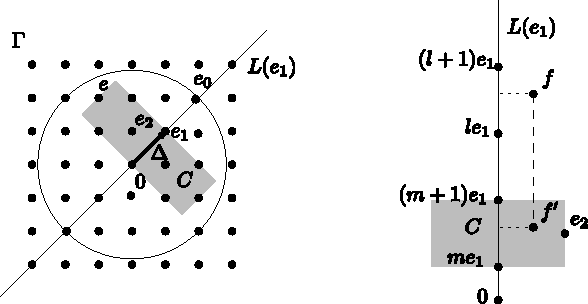
\includegraphics[width=0.8\textwidth]{pics/grupo.pdf}
    \caption{\small Idea de la demostración del lema.}
    \label{fig:grupo}
  \end{figure}

  Ahora, $\{n_1e_1+n_2e_2 \mid (n_1,n_2) \in \ZZ^2 \}$ forma una red discreta en $L(e_1,e_2)$. Además, si existiera un $e\in L(e_1,e_2)\cap \Gamma$ que no perteneciese a la red, podríamos tomar $m_1=[\esc{e}{e_1}]$, $m_2=[\esc{e}{e_2}]$ (donde $[\bullet]$ denota la parte entera). Entonces, $e-m_1e_1-m_2e_2$ estaría más cerca de $L(e_1)$ que $e_2$. Por tanto, esta red es exactamente $L(e_1,e_2) \cap \Gamma$.

      Procedemos ahora por inducción, supongamos que existen $e_1,\dots,e_k$ linealmente independientes tales que $\{n_1e_1+\cdots+n_ke_k \mid (n_1,\dots,n_k) \in \ZZ^k \} = L(e_1,\dots,e_k) \cap \Gamma$ y que existe $e\in \Gamma$ tal que $e \not\in L(e_1,\dots,e_k)$. Análogamente, la proyección ortogonal de $e$ sobre $L(e_1,\dots,e_k)$ cae sobre un hipercubo $\Delta=[m_1e_1,(m_1+1)e_1) \times \cdots \times [m_ke_k,(m_k+1)e_k)$. Si $C$ denota el conjunto de los puntos cuyas proyecciones ortogonales caen en $\Delta$ y son más o igualmente cercanos a $\Delta$ que $e$, entonces $C \cap \Gamma$ es finito. Sea $e_{k+1}$ el más cercano a $\Delta$ de estos puntos, que no esté en $\Delta$. Para cualquier otro $f \in \Gamma$, la distancia entre $f$ y $L(e_1,\dots,e_k)$ es mayor que entre $e_2$ y $L(e_1,\dots,e_k)$, por un razonamiento completamente análogo al caso bidimensional. 

	Por tanto, $\{n_1e_1+\dots+n_{k+1}e_{k+1} \mid (n_1,\dots,n_{k+1}) \in \ZZ^{k+1}\}$ forma una red discreta en $L(e_1,\dots,e_{k+1})$ y, de forma análoga al caso anterior, esta red agota los puntos de $\Gamma\cap L(e_1,\dots,e_{k+1})$.
	Finalmente, sea $k$ el mínimo número natural tal que no existe $e \in \Gamma \backslash L(e_1,\dots,e_k)$. Evidentemente, sabemos que este $k$ existe porque $\RR^n$ es un espacio vectorial de dimensión finita. Entonces $\Gamma$ es isomorfo a $\ZZ^k$.
\end{proof}

Terminamos ahora la demostración del Lema \ref{lemtoro}.
 
  Sea $k$ el número de generadores de $\Gamma$ y sea la proyección natural
  \[
    \begin{array}{rcl}
      \varpi: \RR^n = \RR^k \times \RR^{n-k} & \longrightarrow & \TT^k \times \RR^{n-k} \\
      (x,y) & \longmapsto & (\exp(x), y),
    \end{array}
  \]
  donde la función
  \begin{align*}
    \exp :\RR^k&\longrightarrow \TT^k \cong \SF^1 \times \cdots \times \SF^1\\ 
    (x_1,\dots,x_k) &\longmapsto (e^{i2\pi x_1},\dots,e^{i 2\pi x_k}), 
    \end{align*}
    denota el recubridor universal de $\TT^k$.
  El núcleo de este homomorfismo de grupos $\varpi$ es precisamente el subgrupo $\ZZ^k\subset \RR^n$ generado por los $k$ primeros vectores de la base canónica.. 
  Sean $e_1,\dots,e_k$ los generadores de $\Gamma$ y sea $\zeta:\RR^n \rightarrow \RR^n$ un isomorfismo lineal que mande el $i$-ésimo vector de la base canónica a $e_i$. Entonces, la aplicación $\tilde{\zeta}$ que hace el siguiente diagrama conmutativo es un difeomorfismo,
  \begin{center}
    \begin{tikzcd}
      \RR^n    \arrow{r}{\zeta}\arrow{dd}[anchor=east]{\varpi} & \RR^n\arrow{dd}[anchor=west]{\pi}\arrow{ddr}[rotate=-30]{g} \\ 
  & \\
  \TT^k \times \RR^{n-k}\arrow{r}[anchor=south]{\tilde{\zeta}} & \RR^n/\Gamma \arrow{r}{\tilde{g}}& N
     \end{tikzcd}
   \end{center}
\end{proof}

Volvemos ahora a la demostración del teorema de Arnold-Liouville. Aplicamos directamente el lema \ref{lemtoro} con $N=M_a$ (considerando los campos $X_i=X^{F_i}$ ya definidos y construyendo $g$ como en la demostración del lema) y tenemos que $M_a$ es difeomorfa a $\TT^k\times \RR^{n-k}$ para cierto $k=0,\dots,n$. En particular, si $M_a$ es compacta, entonces $k=n$ y $M_a\cong \TT^n$. Hemos probado entonces la parte $2$ del teorema. Además, el difeomorfismo $\tilde{\zeta}:\TT^k\times \RR^{n-k} \rightarrow M_a$ está bien descrito por el diagrama anterior.

   Podemos considerar entonces la parametrización $\psi:\RR^n\rightarrow M_a$ dada por el diagrama
  \begin{center}
    \begin{tikzcd}
      \RR^n    \arrow[bend left=90]{rrdd}{\psi} \arrow{r}{\zeta}\arrow{dd}[anchor=east]{\varpi} & \RR^n\arrow{dd}[anchor=west]{\pi}\arrow{ddr}[rotate=-30]{g} \\ 
  & \\
  \TT^k \times \RR^{n-k}\arrow{r}[anchor=south]{\tilde{\zeta}} & \RR^n/\Gamma \arrow{r}{\tilde{g}}& M_a,
     \end{tikzcd}
   \end{center}
   Sea el vector $v(a)\in \RR^n$ tal que $\zeta(v(a))=(1,0,\dots,0)$. Tomemos ahora un flujo rectilíneo
   \begin{align*}
      \RR&\longrightarrow \RR^n\\ 
       t &\longmapsto  v(a)t,
     \end{align*}
   y veamos su comportamiento en el diagrama 
   \begin{center}
     \begin{tikzcd}
       t\arrow{rr}\in \RR &&v(a)t \in \RR^n      \arrow{rr}{\zeta}\arrow{rrdd}[anchor=north,rotate=-30]{\psi} && (t,0,\dots,0) \in \RR^n\arrow{dd}[anchor=west]{g} \\ 
 &&       && \\
&&	&&g_{1,t}(x)=\varphi_t^H(x)\in M_a.
      \end{tikzcd}
    \end{center}
    Tenemos entonces que $\varphi_t^H(x)=\psi(v(a)t)$, de modo que podemos tomar una carta $(U,w)$ con $U\subset M_a$ abierto relativo tal que el siguiente diagrama conmute
    \begin{center}
      \begin{tikzcd}
	& & \RR^n \arrow{d}{\psi} \\
	\RR \arrow{r}{\varphi_{\bullet}^H(x)}& U \arrow[hook]{r}{ }\arrow{ru}{w} & M_a.
       \end{tikzcd}
     \end{center}
     Por tanto, $w(t)=w(\varphi_t^H(x))=v(a)t$, luego $\dot w(t)=v(a)$. Como el flujo hamiltoniano deja $M_a$ invariante, queda descrito por las ecuaciones
 \begin{equation*}
   \begin{cases}
     F(t)=a \\
     w(t)=v(a)t.
   \end{cases}
 \end{equation*}
Esto prueba la parte $3$ y por tanto concluye la demostración del teorema.
 \end{proof}

 \begin{obs}
   \em
   Para finalizar la sección vamos a hacer un pequeño comentario sobre la completitud de los campos. Recordemos de la definición \ref{integrable} que una de las cosas que exigíamos a un sistema para que fuera integrable en el sentido de Liouville es que los campos $X^{F_i}$ fueran completos. Sin embargo, en la demostración del teorema de Arnold-Liouville hemos usado algo ligeramente más débil: sólo necesitamos que los campos sean completos en el conjunto de nivel $M_a$. En particular, si nos encontramos ante un toro de Liouville, es decir, si $M_a$ es compacta, entonces todos los campos son completos en $M_a$.
   
   Una garantía segura de la completitud de los campos es que $M$ fuera compacta. Sin embargo en la mayoría de los casos con sentido físico esto no se cumple, pues $M$ suele ser un fibrado tangente, que claramente no es compacto. Por otra parte, el resultado expuesto en \cite{puta} asegura que un campo hamiltoniano $X^G$ es completo en toda la variedad si $G$ es propia, esto es, si la imagen inversa de un compacto por $G$ es un conjunto compacto y si $G$ está acotada inferiormente. De nuevo, esto no aporta gran cosa, pues si las $F_i$ son propias, entonces $F^{-1}(a)$ es compacto y otra vez estaríamos exigiendo que todos los conjuntos de nivel fueran toros de Liouville, aunque esta vez al menos no requerimos que $M$ sea compacta.
 \end{obs}

 \section{Variables de acción-ángulo}
 Vamos a ver el resultado que, junto con el teorema de Arnold-Liouville (y de hecho, en gran parte de la literatura incluido dentro de éste) constituye el núcleo de la teoría de sistemas integrables. En el caso en que $M_a$ sea compacta y, por tanto, un toro de Liouville, vamos a ver que es posible encontrar un entorno de este toro y unas coordenadas (variables de acción-ángulo) en este entorno que nos permitan integrar el sistema por cuadraturas.
 
 Las variables de acción-ángulo fueron introducidas originalmente por Delaunay en 1860 para estudiar el movimiento de la Luna y más tarde, a principios del siglo XX, usadas por los físicos para estudiar el átomo de Bohr. Sería Schwarzschild quien acuñara esa terminología en 1916. La demostración del teorema de las variables de acción-ángulo se atribuye a Mineur en 1936. 

 \begin{thm}[Variables de acción-ángulo]
   Seguimos en las hipótesis del teorema \ref{arnold}. En el caso en que $M_a$ sea compacta, existe un entorno $U\subset M$ de $M_a$ difeomorfo a $\RR^n \times \TT^n$ (un \emph{entorno tubular}\footnote{Nótese que aquí estamos suponiendo que $M_a$ no está en el borde de $M$, en cuyo caso procederíamos análogamente para obtener un entorno difeomorfo a $\HH^n \times \TT^n$.})
) y un sistema de coordenadas de Darboux $(\phi,F)$ (llamadas \emph{variables de acción-ángulo}) en $U$ tales que las $\phi_i$ son coordenadas angulares en $M_a$ y las $F_i$ son constantes en cada $M_a$. 
  \end{thm}

  \begin{obs}
    \em
    La consecuencia inmediata de este teorema es que en los entornos tubulares las ecuaciones de Hamilton quedan resueltas por cuadraturas. En efecto, al ser $(\phi,F)$ coordenadas de Darboux, podemos escribir las ecuaciones de Hamilton en la forma
    \begin{equation*}
      \begin{cases}
	\dot{F_i}=\parcial{H}{\phi_i}, \\
	\dot{\phi_i}=-\parcial{H}{F_i}. 
      \end{cases}
    \end{equation*}
    Ahora, como las $F_i$ son constantes en los toros, se tiene $\dot{F_i}=0$, de modo que $\parcial{H}{\phi_i}$ es constante en cada toro, luego el hamiltoniano no depende de las coordenadas $\phi$. Por tanto, las frecuencias $\nu_i=\dot{\phi_i}=-\parcial{H}{F_i}$ son constantes en cada toro. Así, las ecuaciones quedan integradas en la forma
    \begin{equation*}
      \begin{cases}
	F_i(t)=F_i(0), \\
	\phi_i(t)=\phi_i(0)+\nu_i t. 
      \end{cases}
    \end{equation*}
  \end{obs}

\begin{proof}
  En primer lugar, hay que obtener el entorno tubular $U$. Como $M_a$ es un conjunto compacto de puntos regulares existe un entorno $W$ de $M_a$ con todos sus puntos regulares de manera que $M_a\subset W \subset \overline{W}$ y tal que $F|_W$ sea abierta. Por tanto, $V=F(W)\subset \RR^n$ es un entorno abierto de $a$. Ahora, para cada $b\in V$, existe al menos una componente conexa $M_b$ de $F^{-1}(b)$ que interseca a $W$ en algún punto. Si $M_b$ está contenida en $W$ entonces es compacta y por tanto es un toro de Liouville. En caso contrario, existe un punto $x_b\in M_{b}\cap (\overline{W}\setminus W)$.
  
  Supongamos entonces que existe una sucesión $(b_k)$ de valores en $V$ tal que $b_k\rightarrow a$ con $M_{b_k}\cap(\overline{W}\setminus W) \neq \varnothing$. Entonces existe una sucesión convergente $(x_{b_k})$ con cada $x_{b_k}\in M_{b_k}\cap \overline{W}\setminus W$. Ahora, si llamamos $x_0=\lim_k x_{b_k}$ entonces $x_0\in \overline{W}\setminus W$ y por continuidad $F(x_0)=\lim_k F(x_{b_k})=\lim_k b_k =a$, de modo que $x_0 \in M_a\subset W$ y llegamos a una contradicción. Por tanto existe una bola $B\subset \RR^n$ centrada en $a$ tal que hay algún toro de Liouville $M_b\subset W \subset W$ para cada $b\in B$. 
  
  Podemos considerar entonces el abierto 
  \begin{equation*}
    U=F^{-1}(B)=\bigcup_{b\in B}M_b,
  \end{equation*}
  que es una unión disjunta de toros de Liouville. Ahora, análogamente a la demostración del teorema de Arnold-Liouville, para cada $b\in B$, fijamos $x\in M_b$ y consideramos la aplicación
  \begin{align*}
    \varphi^F :\RR^n&\longrightarrow M_b\\ 
    (\theta_1,\dots,\theta_n) &\longmapsto \varphi_{\theta_1}^{F_1}\cdots \varphi_{\theta_n}^{F_n}(x), 
    \end{align*}
    que está bien definida por conmutar los flujos, y el difeomorfismo $\theta_b:M_b\rightarrow \TT^n$ inducido dado por el diagrama
    \begin{center}
      \begin{tikzcd}
\RR^n	\arrow{r}{\varphi^F}\arrow{d}{ } & M_b\arrow{ld}[anchor=north,rotate=30]{\theta_b} \\ 
	 \TT^n.&
       \end{tikzcd}
     \end{center}
     Tenemos entonces que la aplicación
     \begin{align*}
       \Phi :U&\longrightarrow B\times \TT^n\\ 
       x &\longmapsto (F(x),\theta_{F(x)}(x)), 
       \end{align*}
       es un difeomorfismo. De modo que, como $B$ es una bola, el entorno $U$ es un entorno tubular.

 Procedamos ahora a hallar las variables de acción-ángulo. Sea $\pi:U\cong B\times \TT^n\rightarrow B$ la proyección canónica. Entonces $\pi^{-1}(x)$ es un toro invariante para cada $x \in B$. En cada uno de estos toros, consideramos $X_i=X^{F_i}$ y $(F,\theta)$ las coordenadas antes obtenidas. Si tomamos un punto $\theta=(\theta_1,\dots,\theta_n)\in \RR^n$ entonces, para cada $x\in M$, podemos usar la conmutatividad de los flujos para escribir
\[
  \left. \deriv{\theta_i}\right|_{\varphi^F_{\theta}(x)} = \deriv{\theta_i} \varphi^{F_i}_{\theta_i}(y),
\]
con $y=\varphi^{F_1}_{\theta_1}\cdots\varphi^{F_{i-1}}_{\theta_{i-1}}\varphi^{F_{i+1}}_{\theta_{i+1}}\cdots\varphi^{F_{n}}_{\theta_{n}}(x)$. Ahora, como $\varphi^{F_i}$ es el flujo de $X_i$,
\begin{equation*}
  \left. \deriv{\theta_i}\right|_{\varphi^F_t(x)} = \deriv{\theta_i} \varphi^{F_i}_{\theta_i}(y)=X_{i, \varphi^{F_i}_{\theta_i}(y)}=X_{i,\varphi^F_{\theta}(x)}.
\end{equation*}
De modo que $\deriv{\theta_i}=X_i$.

Como $\omega$ se anula en el toro, no tiene términos en $\dd \theta_i \wedge \dd \theta_j$ y los términos en $\dd F_i \wedge \dd \theta_j$ serán
\[
  \omega\left(\deriv{F_i},\deriv{\theta_j}\right)=\omega\left(\deriv{F_j},X_i\right)=\dd F_i\left(\deriv{F_j}\right)=\delta_{ij}.
\]
Por tanto, $\omega$ es de la forma
\[
  \omega = \sum_{i}^n  \dd F_i \wedge \dd \theta_i + \sum_{k,l=1}^n a_{kl} \dd F_k \wedge \dd F_l,
\]
con $a_{kl}$ unas ciertas funciones. Además, como $\omega$ es cerrada, al diferenciar, cada término correspondiente a $\dd \theta_j \wedge \dd F_k \wedge \dd F_l$ debe anularse. Este término es exactamente
  $\parcial{a_{kl}}{\theta_j}$,
de modo que las $a_{kl}$ son constantes en cada toro invariante.

Si ahora definimos $\alpha=\sum_{i,j=1}^n a_{ij}\dd F_i \wedge \dd F_j$,
\[
  \omega=\sum_{i=1}^n \dd F_i \wedge \dd \theta_i + \alpha.
\]
Como las $a_{ij}$ son constantes en cada toro invariante podemos ver $\alpha$ como  una forma en $\RR^n$, es decir, existe una 2-forma $\beta$ en $\RR^n$ tal que
  $\alpha=\pi^* \beta$.
De aquí tenemos
\[
  0=\dd \omega= \sum_{i=1}^n \dd(\dd F_i \wedge \dd \theta_i) + \dd \alpha= \dd \alpha = \pi^* \dd \beta,
\]
de donde concluimos que $\dd \beta =0$. En $\RR^n$ todas las formas cerradas son exactas, luego existe $\gamma$ en $\RR^n$ tal que $\beta= \dd \gamma$.
Ahora, si escribimos $\gamma= \sum_{i=1}^n f_i \dd F_i$, para algunas funciones $f_i:\RR^n \rightarrow \RR$, entonces podemos tomar unas nuevas coordenadas 
\[
  \phi_i= \theta_i + f_i \circ \pi.
\]
En estas nuevas coordenadas
\[
\begin{split}
  \sum_{i=1}^n \dd F_i \wedge \dd \phi_i & = \sum_{i=1}^n \dd F_i \wedge \dd \theta_i + \sum_{i=1}^n \dd F_i \wedge \dd(f_i \circ \pi)  \\
   & =\sum_{i=1}^n \dd F_i \wedge \dd \theta_i + \pi^* \dd \gamma = \sum_{i=1}^n \dd F_i \wedge \dd \theta_i + \alpha = \omega.
\end{split}
\]

Por tanto, hemos encontrado unas coordenadas de Darboux $(\phi,F)$, con las $F_i$ constantes en cada toro invariante y con las $\phi_i$ coordenadas angulares en estos toros. 
\end{proof}

\begin{obs}
  \em
  En la práctica, las variables de acción-ángulo no suelen obtenerse como en la demostración del teorema. Normalmente se suele trabajar en el fibrado tangente $M=TN$ de cierta variedad riemanniana $N$ de dimensión $n$ en la que se define un sistema lagrangiano natural, igual que hicimos en la sección \ref{sec:fisica}. En este caso, si $(\phi,J)$ son unas variables de acción-ángulo en $M$, se puede escribir
\begin{equation*}
  \omega=\sum_{i=1}^n \dd J_i \wedge \dd \phi_i = \dd \alpha,
\end{equation*}
con $\alpha=\sum_{i=1}^n J_i \dd \phi_i$. Si ahora tomamos los ciclos $\gamma_i$ en los que están definidas las variables $\phi_i$, entonces, como las $J$ no dependen de las $\phi$
\begin{equation*}
  \int_{\gamma_i} \alpha = \sum_{j=1}^n J_j \int_{\gamma_i}\dd \phi_i = \sum_{j=1}^n J_j 2\pi \delta_{ij}= 2\pi J_i.
\end{equation*}
Además, por la independencia de las $\phi$, cada uno de los caminos $\gamma_i$ ha de corresponder a un generador distinto del grupo fundamental del toro de Liouville que estemos tratando.
Así, el procedimiento a seguir para construir variables de acción-ángulo es el siguiente:
\begin{enumerate}
  \item Se toman unas coordenadas de Darboux $(q,p)$ en las que ya se conozca la forma del sistema.
  \item Se hallan los toros de Liouville y se escogen unos ciclos $\gamma_1,\dots,\gamma_n$ que generen el grupo fundamental del toro de Liouville $M_a$ en el que queramos trabajar.
  \item Se obtienen las variables de acción siguiendo la fórmula
    \begin{equation*}
      J_i(a)=\int_{\gamma_i} \sum_{i=1}^n p_i \dd q_i.
    \end{equation*}
  \item Se escribe el hamiltoniano en función de las variables de acción $H=H(J(a))$ y se obtienen las frecuencias 
    \begin{equation*}
      \nu_i(a)= \dot{\varphi_i}(t)=\parcial{H}{J}(J(a)).
    \end{equation*}
\end{enumerate}
\end{obs}

En los ejemplos que veremos a continuación estudiaremos algún caso donde podemos realizar el cálculo explícito de las variables de acción-ángulo y la integración del sistema por cuadraturas.

\section{Osciladores armónicos}
Para aclarar algunas de las ideas detrás de la teoría de sistemas integrables, vamos a considerar uno de los ejemplos más sencillos pero más ilustrativos, el oscilador armónico.

\paragraph{\bf Oscilador armónico con un grado de libertad}\mbox{}

  Empezamos considerando el oscilador armónico con un grado de libertad. El espacio de fases del sistema será el espacio simpléctico estándar $2$-dimensional, $(\RR^2,\Omega_1)$ con las coordenadas de Darboux canónicas $(q,p)$. El hamiltoniano vendrá dado por la función
  \begin{equation*}
    H(q,p)=\tfrac{1}{2}p^2+\tfrac{1}{2}\omega^2 q^2,
  \end{equation*}
  con $\omega$ una constante que representa la frecuencia de oscilación.
  Las ecuaciones de Hamilton son entonces
  \begin{equation*}
    \begin{cases}
      \dot q(t) = \parcial{H}{p}(t)=p(t)\\
    \dot p(t) = -\parcial{H}{q}(t)=-\omega^2q(t).
  \end{cases}
  \end{equation*}
  Estas ecuaciones se pueden integrar fácilmente, si tomamos como condición inicial $(q(0),p(0))=(a,0)$, tenemos
  \begin{equation*}
    \begin{cases}
   q(t)=a\cos\omega t \\ 
   p(t)=-\omega a\sin\omega t.
 \end{cases}
  \end{equation*}
  
  Ahora, recordemos que el hamiltoniano del sistema es una cantidad conservada, por tanto podemos considerar las variedades $M_E$ de energía constante, que, por el teorema de Arnold-Liouville serán topológicamente circunferencias invariantes bajo el flujo del sistema, ya que el único punto crítico del hamiltoniano es su mínimo $(q,p)=(0,0)$. En efecto, las curvas de energía constante vienen dadas por la ecuación
  \begin{equation*}
    E=\tfrac{1}{2}p^2+\tfrac{1}{2}\omega^2q^2,
  \end{equation*}
  que define una elipse de semiejes $\sqrt{2E}$ y $\frac{\sqrt{2E}}{\omega}$. El flujo en las curvas de energía constante toma la forma
  \begin{equation*}
    \begin{cases}
      q(t)=\frac{\sqrt{2E}}{\omega}\cos\omega t \\ 
      p(t)=-\sqrt{2E}\sin\omega t.
 \end{cases}
  \end{equation*}
  
  \begin{figure}[h]
    \centering
    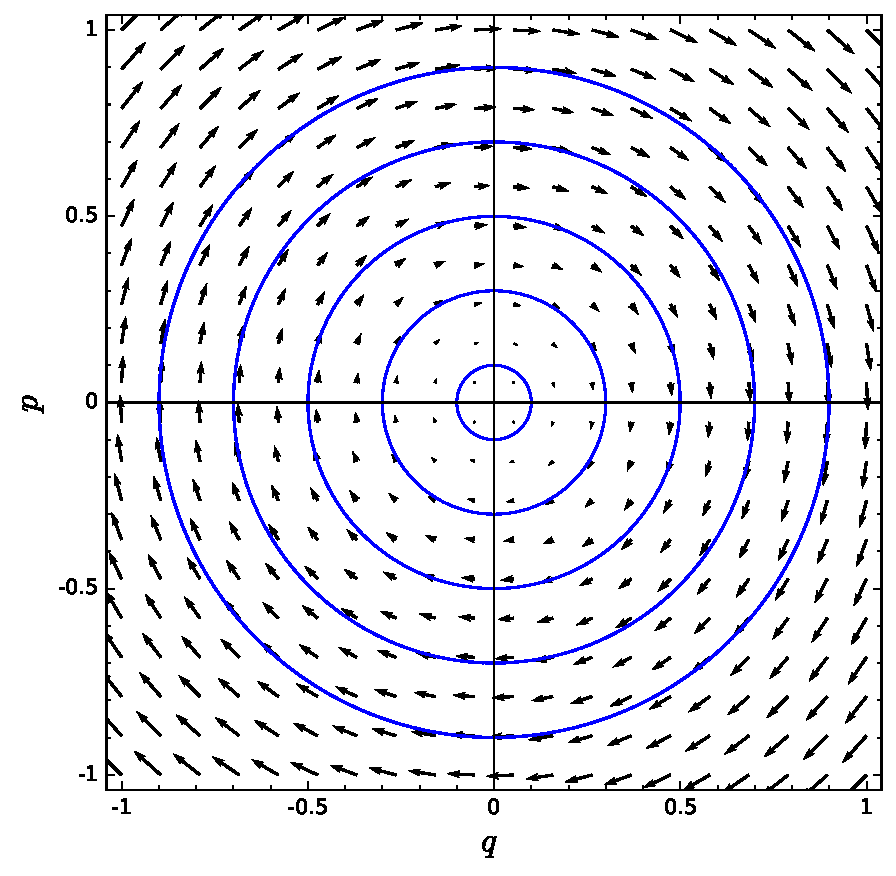
\includegraphics[width=0.8\textwidth]{pics/oscilador}
    \label{fig:oscilador}
    \caption{\small Espacio de fases del oscilador armónico junto al campo y a las curvas de energía constante. En este caso $k=m=1$, de modo que las curvas de energía constante son circunferencias de radio $\sqrt{2E}$.}
  \end{figure}

  Ahora, si tomamos unas coordenadas «polares» $(E,\phi)$, donde $\phi$ es la coordenada angular en cada una de estas elipses, la dinámica del sistema queda mucho más simplificada: 
  \begin{equation*}
    \begin{cases}
    E(t)=E(0) \\
    \phi(t)=\phi(0)-\omega t.
  \end{cases}
  \end{equation*}
  Sin embargo, ¿será canónica la transformación $(q,p) \rightarrow (E,\phi)$? Para ello, veamos cómo se comporta la forma $\Omega_1=\dd p\wedge \dd q$ con el cambio
  \begin{equation*}
    \begin{cases}
      q(E,\phi)=\frac{\sqrt{2E}}{\omega}\cos\phi\\
      p(E,\phi)=\sqrt{2E}\sin \phi.
    \end{cases}
  \end{equation*}
  Tenemos entonces
  \begin{equation*}
    \begin{cases}
      \dd q= \frac{1}{\omega \sqrt{2E}}\cos \phi \dd E - \frac{\sqrt{2E}}{\omega} \sin \phi \dd \phi \\
      \dd p= \sqrt{\frac{1}{2E}}\sin \phi \dd E + \sqrt{2E} \cos \phi \dd \phi,
    \end{cases}
  \end{equation*}
  y 
  \begin{equation*}
    \Omega_1= \dd p \wedge \dd q = -\tfrac{1}{\omega} \dd E \wedge \dd \phi.
  \end{equation*}
  Por tanto, si definimos la \emph{variable de acción}, $J=-\frac{E}{\omega}$, entonces $\Omega_1=\dd J \wedge \dd \phi$ y $(\phi,J)$ son unas coordenadas de Darboux.

  Para tratar de dar sentido físico a esta variable $J$, consideremos el área $A_E$ de la región $S_E$ encerrada por la curva de energía constante $M_E$. Por la fórmula del área de la elipse
  \begin{equation*}
    A_E=\pi \sqrt{2mE} \sqrt{\frac{2E}{k}}=2\pi \sqrt{\frac{m}{k}} E= 2 \pi \frac{E}{\omega}= -2\pi J.
  \end{equation*}

  Observemos ahora que como $\Omega_1$ es la forma de área en $\RR^2$, 
  \begin{equation*}
    A_E=\int_{S_E}\Omega_1 = \int_{S_E} \dd p \wedge \dd q = \int_{M_E}p\dd q,
\end{equation*}
donde hemos usado el teorema de Stokes y el hecho de que $\dd p \wedge \dd q= \dd(p\dd q)$. De modo que podemos redefinir la variable de acción en la forma
\begin{equation*}
  J=-\frac{1}{2\pi}\int_{M_E}p \dd q.
\end{equation*}
Este será el aspecto que tengan las variables de acción-ángulo en general para sistemas con un grado de libertad. Regresando ahora a las coordenadas originales, tenemos
\begin{equation*}
  \begin{cases}
    q(\phi,J)=\sqrt{-\frac{2J}{ \omega}}\cos \phi\\
    p(\phi,J)=\sqrt{-2\omega J}\sin \phi.
  \end{cases}
\end{equation*}

\paragraph{\bf Oscilador armónico con $n$ grados de libertad}\mbox{}

  Para estudiar un caso de dimensión superior, podemos considerar el sistema formado por $n$ osciladores armónicos acoplados o, equivalentemente, un oscilador armónico con $n$ grados de libertad. El hamiltoniano del sistema será 
  \begin{equation*}
    H(q_1,\dots,q_n,p_1,\dots,p_n)= H_1(q_1,p_1)+ \cdots +H_n(q_n,p_n) = \tfrac{1}{2}\sum_{i=1}^n (p_i^2+\omega_i^2q_i^2).
  \end{equation*}
  Este sistema es integrable en el sentido de Liouville. Basta tomar $F=(H_1,H_2,\dots,H_n),$ ya que 
  \begin{equation*}
    \pois{H_i}{H_j} = \sum_{k=1}^n\left( \parcial{H_i}{p_k}\parcial{H_j}{q_k} - \parcial{H_j}{p_k}\parcial{H_i}{q_k}\right)=0
  \end{equation*}
  y las componentes de $F$ son independientes en casi todo punto de $\RR^{2n}$. 
  
  Ahora, dado $a=(a_1,\dots,a_n)\in \RR^n$, $M_a=F^{-1}(a)$ vendrá dado por 
  \begin{align*}[left=\empheqlbrace]
      p_1^2+\omega_1^2q_1^2&=2a_1 \\
      p_2^2+\omega_2^2q_2^2&=2a_2 \\
      & \vdotswithin{=} \\
p_n^2+\omega_n^2q_n^2&=2a_n, 
  \end{align*}
  que son las ecuaciones de un toro $n$-dimensional. Cada una de las ecuaciones $p_i^2+q_i^2=2a_i$ da, en el plano $(q_i,p_i)$, una elipse $C_{a,i}$ de semiejes $\sqrt{2a_i}$ y $\frac{\sqrt{2a_i}}{\omega}$, de modo que $M_a=C_{a,1}\times\dots\times C_{a,n}$. Nótese que en este caso los valores críticos son precisamente aquellos $a$ con varias componentes iguales, de forma que los puntos críticos formarán toros de dimensión menor.

  Consideremos $\gamma_{a,i}$ lazos en cada elipse $C_{a,i}$, de manera que los $\gamma_{a,i}$ son generadores del grupo fundamental de $M_a$. Entonces podemos definir las variables de acción 
  \begin{equation*}
    J_i(a) = \frac{1}{2\pi}\int_{\gamma_{a,i}}\sum_{k=1}^n  p_k \dd q_k=\frac{1}{2\pi}\int_{\gamma_{a,i}}  p_i \dd q_i=\frac{a_i}{\omega_i}.
  \end{equation*}

  Consideremos ahora las variables angulares $\phi_i$ a lo largo de cada $C_{i,a}$. Podemos tomar entonces las nuevas coordenadas $(\phi,J)$, con
  \begin{equation*}
    J_i(q,p)=J_i(F(q,p))=\frac{1}{2\pi}\int_{\gamma_{F(q,p),i}} p_i \dd q_i= \frac{H_i(q,p)}{\omega_i},
  \end{equation*}
  y $\phi(q,p)$ las variables angulares en el toro $M_{F(q,p)}$.
  Si la carta $(\phi,J)$ es de Darboux, las ecuaciones de Hamilton pueden integrarse por cuadraturas. Esto se debe a que $H=\sum_{i=1}^n H_i(J,\phi)=\sum_{i=1}^n \omega_i J_i$, de modo que, por las ecuaciones de Hamilton,
\begin{equation*}
  \begin{cases}
  \dot{J_i}=\parcial{H}{\phi_i}=0,\\
  \dot{\phi_i}=-\parcial{H}{J_i} = -\omega_i.
  \end{cases}
\end{equation*}
 Las ecuaciones de Hamilton quedan entonces integradas en la forma
\begin{equation*}
  \begin{cases}
  J_i(t)=  J_i(0) \\
  \phi_i(t) =  \phi_i(0) - \omega_i t.
\end{cases}
\end{equation*}
Este tipo de flujo en el toro se llama \emph{movimiento condicionalmente periódico}, ya que, dependiendo de los valores de las frecuencias $\omega_i$, las trayectorias serán cerradas y periódicas o serán densas en cada toro de Liouville. En la siguiente sección profundizaremos más en este tema.

\section{Movimiento condicionalmente periódico}\label{sec:promedios}
Una vez tenemos a nuestra disposición el teorema de Arnold-Liouville, sabemos que el flujo en los toros de Liouville será muy sencillo. En esta sección vamos a estudiar el flujo en estos toros y obtendremos un teorema muy importante sobre este tipo de sistemas.

  En primer lugar, consideremos un $2$-toro de Liouville. Sea $(\theta_1,\theta_2)$ un punto en el toro y su trayectoria bajo el flujo hamiltoniano $\gamma(t)=\varphi_t(\theta_1,\theta_2)=(\theta_1+\omega_1t,\theta_2+\omega_2t)$. Si $\omega_1/\omega_2=m/n$ es racional, entonces 
  \begin{equation*}
    \gamma\left(\frac{2n\pi}{\omega_2}\right) = (\theta_1+2m\pi,\theta_2+2n\pi)=(\theta_1,\theta_2).
  \end{equation*}
  Es decir, a cierto tiempo la trayectoria «se cierra». Estas órbitas se dicen \emph{periódicas}. 
 
  Sin embargo, si $\omega_2/\omega_1$ es irracional, dado un ángulo $\alpha$ y tomando $T$ tal que $\alpha=\theta_1+\omega T$, entonces podemos tomar $T_n=T+2n\pi/\omega_1$, $\alpha=\theta_1+\omega_1(T_n)$ para cada $n\in \NN$. Ahora, la aplicación
  \begin{equation*}
    \begin{array}{rcl}
    g:\SF^1 & \longrightarrow &\SF^1 \\
  \phi & \longmapsto & \phi + 2\pi\frac{\omega_2}{\omega_1},
  \end{array}
\end{equation*}
es una rotación de ángulo un múltiplo irracional de $2\pi$ en la circunferencia del toro de ángulo $\alpha$. Entonces, como ya vimos por el teorema de recurrencia de Poincaré (teorema \ref{tpoincare}), $\{g^n(\phi)|n\in \NN\}$ es denso en $\SF^1$. Como esto es válido para todo $\alpha$ y se cumple 
\begin{equation*}
  \gamma(T_n)=(\alpha,g^n(\theta_2)+\omega_2 T),
\end{equation*}
tenemos que $\{\gamma(t)|t \in \RR \}$ es denso en el toro. Este tipo de órbitas se llaman \emph{cuasiperiódicas}. Una forma sencilla de visualizar esto es mediante las \emph{figuras de Lissajous} 
\begin{equation*}
  L_{\omega}=\{(\cos t, \cos \omega t) | t \in \RR\},
\end{equation*}
ver figura \ref{fig:lissajous}.
\begin{figure}[h!]
  \centering
  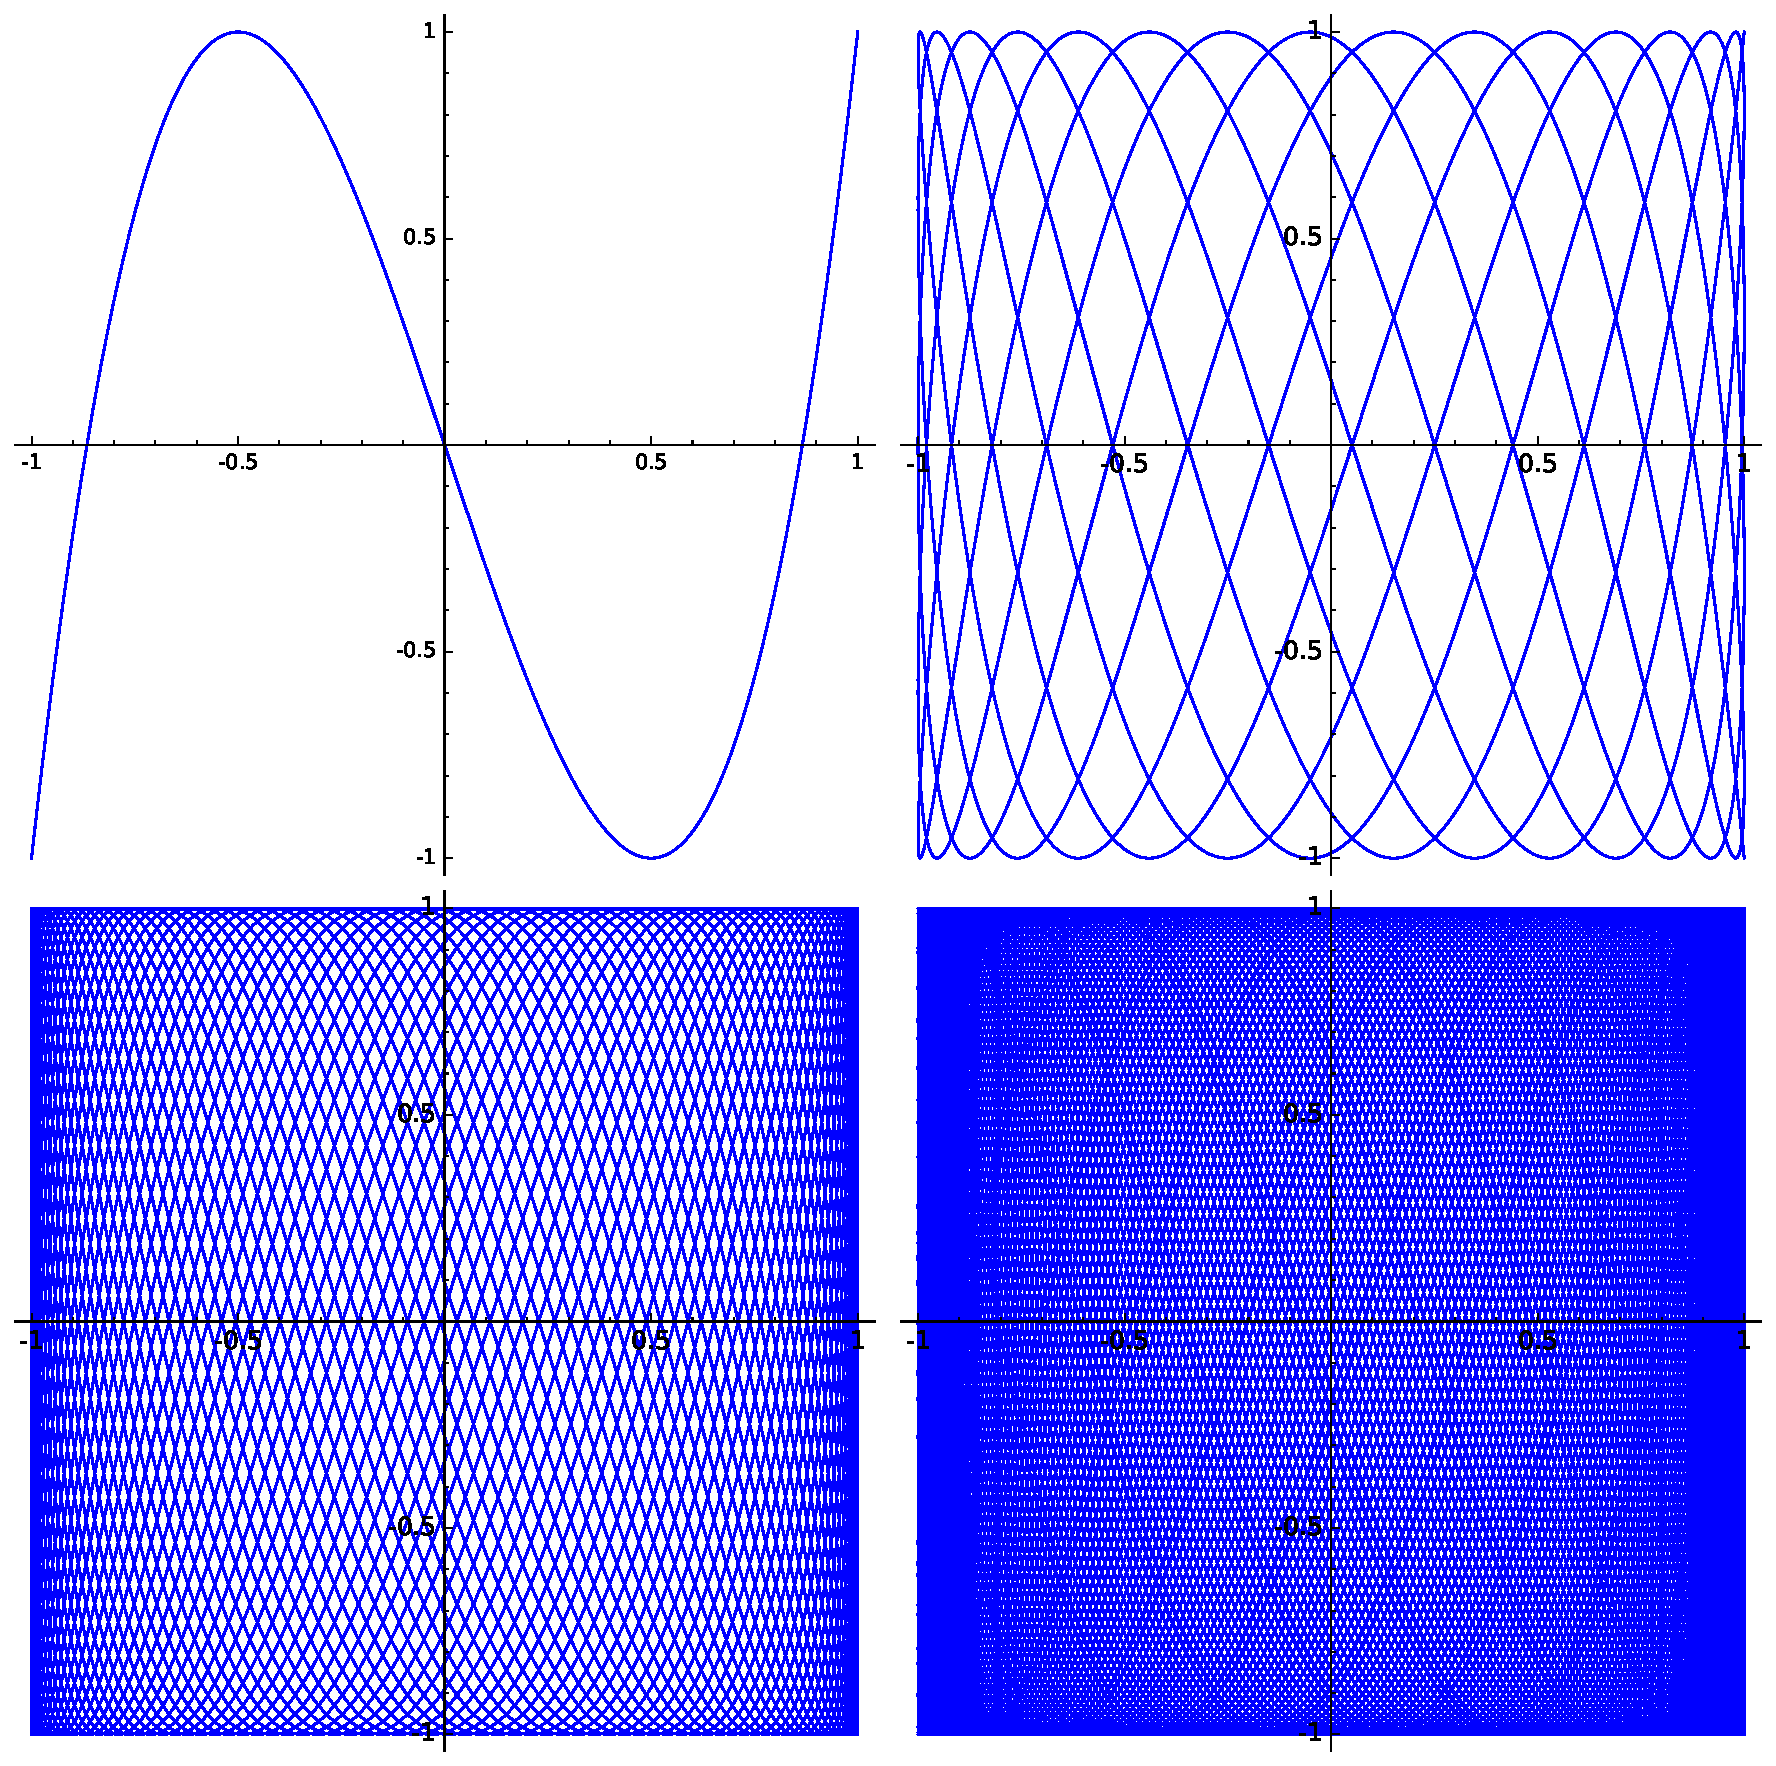
\includegraphics[width=0.8\textwidth]{pics/lissajous}
  \caption{\small Figuras de Lissajous para $\omega=3,$ $3.1,$ $3.14,$  y $3.1416$, $t \in (0,128\pi)$ con pasos de $0.01$.}
  \label{fig:lissajous}
\end{figure}

Vamos a generalizar ahora estas ideas al caso $n$-dimensional.

\begin{defn}
  \em
  Sean $\TT^n$ el toro $n$-dimensional y $\phi=(\phi_1,\dots,\phi_n)$ coordenadas angulares. Se entiende por un \emph{movimiento condicionalmente periódico} en el toro el flujo uniparamétrico dado por 
  \begin{equation*}
    \phi(t)=\phi(0)+\omega t
  \end{equation*}
  con $\omega=(\omega_1,\dots,\omega_n)$ \emph{frecuencias} constantes en el toro. Las frecuencias $\omega$ se dicen \emph{independientes} si, para cada $k \in \ZZ^n$,  $\esc{k}{\omega}=0$ si y sólo si $k=0$.
\end{defn}
\begin{defn}
  \em
  Sea $f:\TT^n \rightarrow \RR$ una función integrable Riemann,
  \begin{enumerate}
    \item El \emph{promedio espacial} de $f$ en $\TT^n$ es el número
      \begin{equation*}
	\bar{f}=\frac{1}{(2\pi)^n}\int_0^{2\pi} \cdots \int_0^{2\pi} f(\phi) d\phi_1,\dots,d\phi_n.
      \end{equation*}
    \item El \emph{promedio temporal} de $f$ en $\TT^n$ es la función
      \begin{equation*}
	f^*(\phi_0)=\lim_{T\rightarrow \infty} \int_0^{T}f(\phi_0+\omega t) dt,
      \end{equation*}
      definida en los puntos $\phi_0$ en los que exista el límite.
  \end{enumerate}
\end{defn}

\begin{thm}[Teorema de los promedios]
  Si $f:\TT^n \rightarrow \RR$ es una función integrable Riemann y las frecuencias $\omega$ son independientes, el promedio temporal está bien definido en todo el toro $\TT^n$ y coincide en todo punto con el promedio espacial.
\end{thm}
\begin{proof}
    En primer lugar, consideramos funciones de la forma $e^{i\esc{k}{\phi}}$, $k\in \ZZ^n$. Si $k=0$, entonces $\bar{f}=f=f^*=1$. Si $k\neq0$, $\bar{f}$ es una integral a periodos en funciones trigonométricas, luego es igual a 0. Por otra parte
     \begin{equation*}
       \int_0^T e^{i\esc{k}{\phi_0 + \omega t}} dt= e^{i\esc{k}{\phi_0}}\int_0^T e^{i\esc{k}{\omega}t}dt=e^{i\esc{k}{\phi_0}}\frac{e^{i\esc{k}{\omega}T}-1}{i \esc{k}{\omega}}.
     \end{equation*}
     Por tanto, el promedio temporal será
     \begin{equation*}
       \lim_{T\rightarrow \infty}\frac{e^{i\esc{k}{\phi_0}}}{i \esc{k}{\omega}}\frac{e^{i\esc{k}{\omega}T}-1}{T}=0.
     \end{equation*}
     
    Como los promedios dependen linealmente de $f$, también coincidirán para los polinomios trigonométricos
     \begin{equation*}
       f=\sum_{|k|<N}f_ke^{i\esc{k}{\omega}}.
     \end{equation*}

    Dado $\varepsilon >0$, si $f$ es continua y real por el teorema de Weierstrass podemos aproximarla por un polinomio trigonométrico $P$ que cumpla $|f-P|<\frac{1}{2}\varepsilon$. Sean $P_1=P-\frac{1}{2}\varepsilon$, $P_2=P+\frac{1}{2}\varepsilon$ entonces
     \begin{equation*}
       \bar{P_2}-\bar{P_1}=\frac{1}{(2\pi)^n}\int_{\TT^n} (P_2 - P_1) d\phi = \frac{1}{(2\pi)^n}\varepsilon (2\pi)^n= \varepsilon.
     \end{equation*}

    Dado $\varepsilon >0$, si $f$ es real e integrable Riemann, entonces existen dos funciones continuas $f_1,f_2$ tales que $f_1<f<f_2$ y $\int_{\TT^n}\frac{1}{(2\pi)^n}(f_2-f_1)d\phi<\frac{1}{3}\varepsilon$. Tomando ahora $P_1,P_2$ polinomios trigonométricos tales que $P_1<f_1<f_2<P_2$ y $\int_{\TT^n}\frac{1}{(2\pi)^n}(P_i-f_i)d\phi < \frac{1}{3}\varepsilon$, para $i=1,2$, entonces
     \begin{equation*}
       \bar{P_2}-\bar{P_1}=\frac{1}{(2\pi)^n}\int_{\TT^n} (P_2 - P_1) d\phi = \frac{1}{(2\pi)^n}\varepsilon (2\pi)^n= \varepsilon.
     \end{equation*}

    Por último, sea $\varepsilon>0$, entonces existen dos polinomios trigonométricos $P_1,P_2$ tales que $P_1<f<P_2$ y $\bar{P_2}-\bar{P_1}<\varepsilon$. Ahora, como $f<P_2$,
     \begin{equation*}
       \frac{1}{T}\int_0^T f(\phi(t))dt < \frac{1}{T}\int_0^T P_2(\phi(t))dt,
     \end{equation*}
     luego
     \begin{equation*}
       \left| \frac{1}{T}\int_0^T f(\phi(t))dt- \bar{f} \right| <\left| \frac{1}{T}\int_0^T P_2(\phi(t))dt- \bar{f} \right| < \left| \frac{1}{T}\int_0^T P_2(\phi(t))dt- \bar{P_2}\right| + |\bar{P_2}-\bar{f}|.
     \end{equation*}
     Pero, como $P_1<f<P_2$, por la monotonía de la integral $\bar{P_1}<f<\bar{P_2}$, luego $|\bar{P_2}-\bar{f}|<|\bar{P_2}-\bar{P_1}|<\varepsilon$. Además, como $P_2$ es un polinomio trigonométrico existe un $T_0$ tal que, si $T>T_0$
     \begin{equation*}
       \left| \frac{1}{T}\int_0^T P_2(\phi(t))dt- \bar{P_2}\right| < \varepsilon .
     \end{equation*}
     Finalmente, obtenemos lo que queríamos probar
     \begin{equation*}
       \left| \frac{1}{T}\int_0^T f(\phi(t))dt- \bar{f} \right| <\left| \frac{1}{T}\int_0^T P_2(\phi(t))dt- \bar{P_2}\right| + |\bar{P_2}-\bar{f}|<\varepsilon + \varepsilon = 2\varepsilon,
     \end{equation*}
     luego $f^*(\phi_0)=\lim_{t\rightarrow \infty}\frac{1}{T}\int_0^T f(\phi(t)) dt = \bar{f}$.
\end{proof}
\begin{corol}
  Si las frecuencias son independientes, entonces, para todo $\phi_0 \in \TT^n$, \[\{\phi(t)=\phi_0+\omega t|t\in \RR\}\] es denso en el toro $\TT^n$.
\end{corol}
\begin{proof}
  En caso contrario, podemos tomar un abierto $D$ del toro que no tiene ningún punto de la trayectoria $\phi(t)$. Construimos la función 
  \begin{equation*}
    f(\phi)=\left\lbrace
    \begin{array}{ll}
      0 & \text{si } \phi \not\in D \\
      \frac{(2\pi)^n}{\int_D d\phi} & \text{si } \phi \in D.
    \end{array}
    \right.
  \end{equation*}
  Claramente, $\bar{f}=1$, pero $f^*(\phi_0)=0$, lo que contradice el teorema de los promedios.
\end{proof}
\begin{corol}
  Sea $D\subset \TT^n$ un conjunto medible Jordan. Sea $A_D=\{t\in \RR | \phi(t) \in D\}$ (que también es medible Jordan) y sea $\tau_D(T)=\int_0^T\chi_{A_D}(t)dt$. Entonces
  \begin{equation*}
    \lim_{T\rightarrow \infty}\frac{\tau_D(T)}{T}= \frac{\mathrm{Vol}(D)}{(2\pi)^n}.
  \end{equation*}
\end{corol}
\begin{proof}
  Aplicamos el teorema a $\chi_D$, entonces $\int_0^T \chi_D(\phi(t))dt=\int_0^T \chi_{A_D}(t)dt=\tau_D(t)$ y $\bar{\chi}_D=(2\pi)^{-n}\mathrm{Vol}(D)$. Finalmente, por el teorema de los promedios
  \begin{equation*}
    \bar{\chi}_D=\frac{\mathrm{Vol}(D)}{(2\pi)^n}=\lim_{T\rightarrow \infty}\frac{1}{T}\int_0^T \chi_D(\phi(t))dt=\lim_{T\rightarrow \infty}\frac{\tau_D(T)}{T}.
  \end{equation*}
\end{proof}
\section{Sistemas con un grado de libertad}
En esta sección damos algunas generalidades sobre los sistemas hamiltonianos con un grado de libertad que, como ya hemos visto, son todos integrables en el sentido de Liouville. Uno de los ejemplos más característicos es el péndulo simple, que estudiamos a continuación.
  
\paragraph{\bf El péndulo simple}\mbox{}
  
  Consideramos un péndulo de masa $m=1$ cuya «cuerda» es una barra rígida de masa despreciable y longitud $1$. El espacio de configuración del péndulo es entonces la circunferencia unidad $\SF^1$ y su espacio de fases será el fibrado tangente de $\SF^1$, que no es otra cosa que un cilindro. Tomando como coordenada generalizada el ángulo $\phi$ de desviación del péndulo respecto de la vertical, el hamiltoniano viene dado por 
  \begin{equation*}
    H(\phi,p)=\frac{1}{2}p^2 - g\cos\phi,
  \end{equation*}
  donde $g$ es la aceleración de la gravedad y hemos tomado el centro como origen de energía potencial.
  Como podemos ver en la figura \ref{fig:pendulo}  las trayectorias son cerradas, luego cada curva de energía constante es compacta. Para estudiar los puntos críticos, nótese que $\dd H$ es distinta de 0 en todo punto exceptuando los casos $(\phi=0,p=0)$ y $(\phi=\pi,p=0)$, que corresponden a puntos de equilibrio (el primero, estable, el segundo, inestable) donde la trayectoria es sólo un punto. La curva que aparece punteada en la figura, de ecuación
  \begin{equation*}
    g=H(\phi,p)=\frac{1}{2}p^2 - g \cos\phi ,
  \end{equation*}
   corresponde al punto de equilibrio y a dos trayectorias que tienden asintóticamente al punto de equilibrio inestable. Este conjunto no es un toro de Liouville ya que contiene al punto crítico $(\pi,0)$. Estas trayectorias son matemáticamente factibles aunque su realización práctica parezca una tarea imposible. Las curvas que quedan dentro de la curva punteada corresponden a movimientos de oscilación en torno al punto de equilibrio estable, mientras que las que quedan fuera corresponden a movimientos de rotación del péndulo alrededor de su centro. 
  \begin{figure}[h]
    \centering
    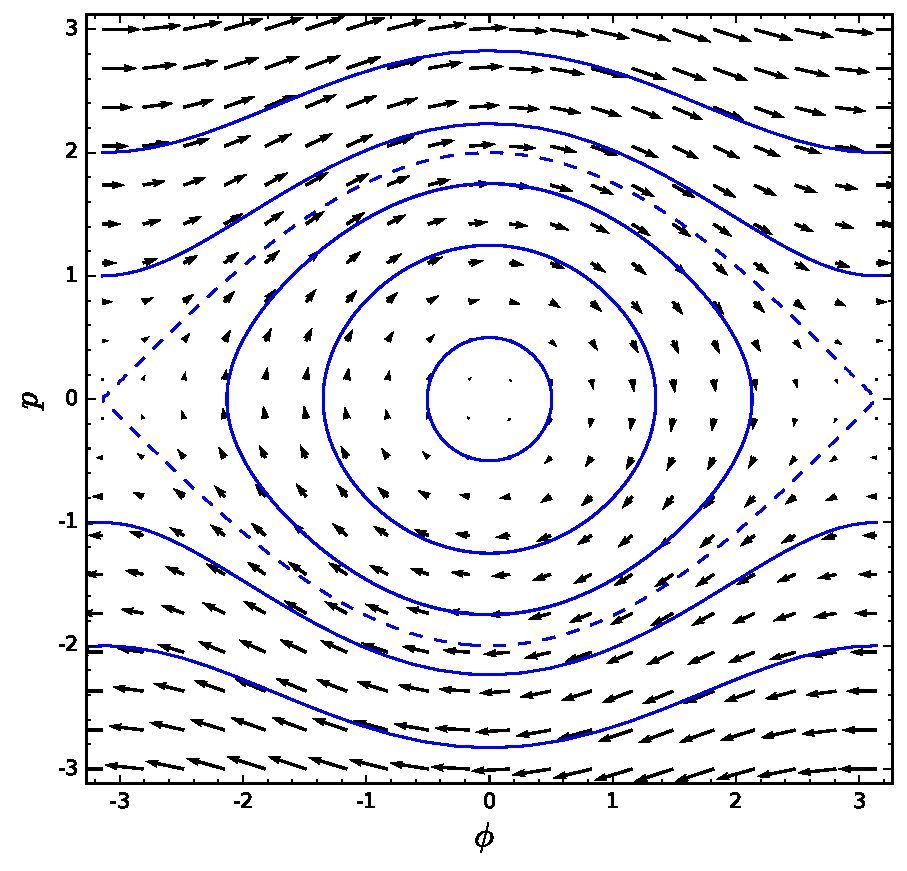
\includegraphics[width=0.8\textwidth]{pics/pendulo}
    \caption{\small Espacio de fases del péndulo junto al campo hamiltoniano y las curvas de nivel. Nótese que el lado derecho ($\phi=\pi$) está identificado con el lado izquierdo ($\phi=-\pi$), ya que se trata de un cilindro.}
    \label{fig:pendulo}
  \end{figure}

   \paragraph{\bf Puntos críticos de los sistemas con un grado de libertad}\mbox{}

   Los dos tipos de punto crítico que presenta el péndulo simple se conocen como \emph{centros}, para el $(0,0)$ y \emph{sillas}, para el $(\pi,0)$. Podemos probar que, de hecho esos son los únicos tipos de punto crítico que puede presentar un sistema hamiltoniano en $\RR^2$. En efecto, supongamos que $(0,0)$ es un punto de equilibrio de un sistema hamiltoniano. Podemos escribir las ecuaciones de Hamilton en la forma
   \begin{equation*}
     \left(
     \begin{array}{c}
       \dot q \\
       \dot p
     \end{array}
     \right)=
\left(
     \begin{array}{cc}
       0 & -1\\
       1 & 0
     \end{array}
     \right)
\left(
     \begin{array}{c}
       \parcial{H}{q} \\
       \parcial{H}{p}
     \end{array}
     \right),
   \end{equation*}
   de modo que su versión linealizada en torno al $(0,0)$ será
   \begin{equation*}
     \left(
     \begin{array}{c}
       \dot q \\
       \dot p
     \end{array}
     \right)=
\left(
     \begin{array}{cc}
       0 & -1\\
       1 & 0
     \end{array}
     \right)
     \left.
\left(
     \begin{array}{cc}
       \frac{\partial^2 H}{\partial q^2} & \frac{\partial^2 H}{\partial p \partial q} \\
       \frac{\partial^2 H}{\partial q \partial p} & \frac{\partial^2 H}{\partial p \partial p} 
     \end{array}
     \right)
     \right|_{(q,p)=(0,0)}
\left(
     \begin{array}{c}
       q \\
       p
     \end{array}
     \right)
     =J_1 B
\left(
     \begin{array}{c}
       q \\
       p
     \end{array}
     \right)
     =A
\left(
     \begin{array}{c}
       q \\
       p
     \end{array}
     \right).
   \end{equation*}
   De la simetría de la matriz de segundas derivadas $B$ y de las propiedades de la matriz $J_1$, tenemos que $A$ ha de cumplir la condición
   \begin{equation*}
     A^{t}J_1+J_1 A=0.
   \end{equation*}
   Las matrices que cumplen esta condición forman el álgebra de Lie $\mathfrak{sp}(2)$ del grupo simpléctico $\mathrm{Sp}(2)$.

   \begin{prop}
     Si $\alpha$ es un autovalor de una matriz $A\in \mathfrak{sp}(2)$ con multiplicidad algebraica $k$, entonces $-\alpha$ es también un autovalor de $A$ con la misma multiplicidad. Si $\alpha=0$ entonces su multiplicidad es par.
   \end{prop}
   \begin{proof}
     Los autovalores son los ceros del polinomio característico $P(\alpha)=\det(\alpha I-A)$. Por tanto, basta probar que $\det(\alpha I-A)=\det(\alpha I + A)$. Esto se ve de la siguiente manera,
     \begin{align*}
       P(\alpha)&=\det(\alpha I-A)=\det(-\alpha J_1^2-J_1B)=\det J_1\det(-\alpha J_1 - B)\\
       &=\det(-\alpha J_1-B)^t=\det (\alpha J_1 - B)=\det(\alpha I - J_1^{-1}B)\\
       &=\det(\alpha I + J_1 B)=\det(\alpha I +A).
     \end{align*}
   \end{proof}
   Por tanto, los autovalores de $A$ son imaginarios, opuestos o ambos cero, luego el punto crítico $(0,0)$ solo puede ser un centro (en el caso de autovalores imaginarios) o un punto de silla (en el caso de autovalores reales opuestos). Como consecuencia de esto tenemos que el sistema hamiltoniano no puede tener puntos \emph{asintóticamente estables}, lo que tal vez era de esperar a la vista de la conservación de la energía y del teorema de Liouville: los puntos asintóticamente estables funcionarían como «fuentes» o «sumideros» del área de Liouville.
   \section{Más sistemas integrables}
   Cuando estudiamos sistemas con varios grados de libertad, la integrabilidad requiere de la existencia de cantidades conservadas adicionales. Como ya vimos en el apartado de simetrías y leyes de conservación, una forma útil de encontrar cantidades conservadas es observar las simetrías del sistema, siguiendo el mecanismo de Noether. En esta sección veremos dos ejemplos donde podemos ver directamente esta relación entre las simetrías y la integrabilidad del sistema.

   \paragraph{\bf El péndulo esférico}\mbox{}

   Un péndulo esférico consiste en una partícula (aquí supondremos de masa $m=1$) enganchada por una barra rígida de masa despreciable y de longitud 1 a un punto del espacio y bajo la acción de la gravedad. Es decir, es como un péndulo simple, solo que no está restringido a oscilar en un solo plano, sino que puede moverse libremente, ver figura \ref{fig:espendulo}.
\begin{figure}[h]
  \centering
  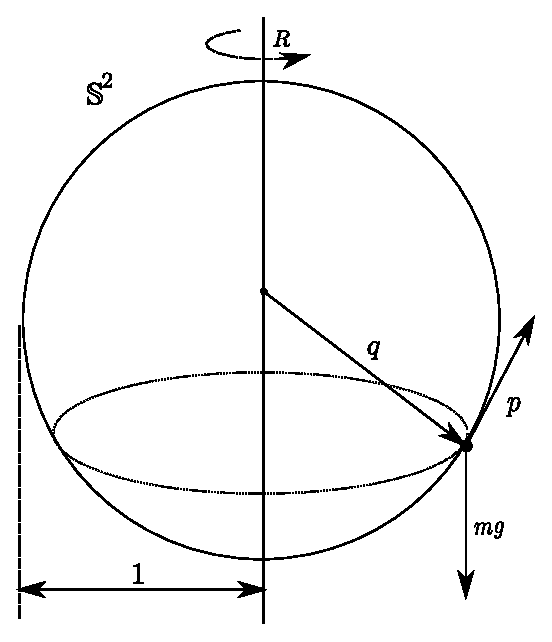
\includegraphics[width=0.5\textwidth]{pics/espendulo.eps}
  \caption{\small Péndulo esférico}
  \label{fig:espendulo}
\end{figure}

Podemos considerar el sistema inmerso en $\RR^3$, de modo que el espacio de fases en principio será el espacio simpléctico estándar $6$-dimensional $(\RR^6,\Omega_3)$. Ahora, la ligadura del péndulo restringe el movimiento espacial a una esfera de radio 1, y las velocidades serán siempre tangentes a esta esfera. De este modo, el espacio de fases será
\begin{equation*}
  M=\left\{ (q,p)\in \RR^6 : ||q||=1, \esc{q}{p}=0 \right\},
\end{equation*}
que claramente es difeomorfo al fibrado tangente de la esfera, $T\SF^2$. La forma simpléctica en $M$ será simplemente la restricción de $\Omega_3$ a $M$. El hamiltoniano será la restricción a $M$ de la función 
\begin{align*}
  H :\RR^6&\longrightarrow \RR\\ 
  (q,p) &\longmapsto \tfrac{1}{2m}||p||^2+mgq_3, 
  \end{align*}
  donde $q_3$ es la componente vertical del vector $q=(q_1,q_2,q_3)$.

  Observemos ahora que el sistema es invariante bajo las rotaciones en torno a la vertical. En efecto, si $R\in\mathrm{SO}(3)$ es una rotación en torno a la vertical, como la tercera componente no varía respecto de las rotaciones en torno a la vertical y las rotaciones preservan la norma,
  \begin{equation*}
    H(R(q),R(p))=\tfrac{1}{2m}||R(p)||^2+mgq_3=\tfrac{1}{2m}||p||^2+mgq_3=H(q,p).
  \end{equation*}
  Por tanto, la tercera componente del momento angular $L_3=q_1p_2-q_2p_1$ es una cantidad conservada del sistema $(M,H)$. Como $\dim(M)=4$ y hemos encontrado una cantidad conservada del sistema a parte del propio hamiltoniano, no es difícil comprobar que $H$ y $L_3$ son independientes para casi todo punto, luego el sistema $(M,H)$ será integrable en el sentido de Liouville.

  \paragraph{\bf El potencial central}\mbox{}

  Consideremos el caso genérico de una partícula moviéndose en el espacio sujeta a una fuerza central, es decir, dirigida siempre hacia el origen y cuyo valor dependa solo de la distancia de la partícula a este. Un ejemplo típico sería el de una partícula moviéndose en un potencial kepleriano $V(r)=-k/r$ (por ejemplo, la Tierra alrededor del Sol). El espacio de fases del sistema es el espacio simpléctico estándar $6$-dimensional $(\RR^6,\Omega_3)$ y el hamiltoniano viene dado por la función
  \begin{equation*}
    H(q,p)=\tfrac{1}{2m}||p||^2+V(||q||).
  \end{equation*}
  Claramente, el sistema es invariante bajo rotaciones ya que, si $R\in \mathrm{SO}(3)$ es una rotación, entonces, como las rotaciones preservan la norma
  \begin{equation*}
    H(R(q),R(p))=\tfrac{1}{2m}||R(p)||^2+V(||R(q)||)=\tfrac{1}{2m}||p||^2+V(||q||)=H(q,p).
  \end{equation*}
  Como consecuencia, se conserva el momento angular $L=q\times p$. En particular, se conservarán $L^2=\esc{L}{L}$ y $L_3=q_1p_2-q_2p_1$. Ahora, si calculamos el corchete de Poisson
  \begin{equation*}
    \pois{L^2}{L_3}=\sum_{i=1}^3\pois{L_i^2}{L_3}=\sum_{i=1}^32L_i\pois{L_i}{L_3},
  \end{equation*}
  por la regla de Leibniz. Como $\pois{L_3}{L_3}=0$, tenemos 
  \begin{equation*}
    \pois{L^2}{L_3}=2L_1\pois{L_1}{L_3}+2L_2\pois{L_2}{L_3}.
  \end{equation*}
  Basta entonces hallar 
  \begin{equation*}
    \pois{L_1}{L_3}=\pois{q_2p_3-q_3p_2}{q_1p_2-q_2p_1},
  \end{equation*}
  que, usando la linealidad del corchete de Poisson y la identidad de Jacobi y teniendo en cuenta que $\pois{q_i}{q_j}=\pois{p_i}{p_j}=0$ podemos desarrollar hasta llegar a
  \begin{equation*}
    \pois{L_1}{L_3}=-p_3q_1\pois{q_2}{p_2}-q_3p_1\pois{p_2}{q_2}=+p_3q_1-q_3p_1=-L_2.
  \end{equation*}
Un cálculo análogo muestra que $\pois{L_2}{L_3}=L_1$, de modo que
\begin{equation*}
  \pois{L^2}{L_3}=-2L_1L_2+2L_2L_1=0.
\end{equation*}

Por tanto, $H$, $L^2$ y $L_3$ son $3$ funciones en involución y además es posible comprobar que son independientes en casi todo punto de $\RR^6$, de modo que el sistema $(M,H)$ es integrable en el sentido de Liouville.

